\chapter{Blockchain-Based Cryptocurrency Network in a Time of Crisis\label{cha:chapter5}}

Blockchain-based cryptocurrencies provide a mechanism for the exchange of value across the internet.
The nature of a public blockchain data-structure is such that a complete record of the transaction history is freely available at all times to all interested parties.
In contrast to traditional econometric approaches this paradigm presents a fundamentally new model for the analysis of dynamic characteristics in a globally distributed network of exchange. 
In this chapter we perform a comprehensive investigation of the distortions and pathologies observable throughout a period of irregular value fluctuation in the transaction network of Bitcoin, a representative cryptocurrency. 
We discover strong structural changes in the dynamical network defined by the transactions between addresses.  
Regions of strong market volatility are characterized by low transitivity in the network. 
Moreover the collapse of the largest financial intermediary and the ensuing crisis this provoked is demonstrated to be clearly discernible solely on the basis of deviations from the Pareto behavior in the degree distribution of the network. 
On the basis of information theory we introduce a new dynamical metric used to quantify volatility fluctuations and measure market anomalies in the network.

\section{Discovered Pathologies}

The global financial crisis of 2008 brought into stark relief the inadequacy of traditional metrics to assess risk. 
This state of affairs can be encapsulated by the headline from January $3^{rd}$ 2009 in the London newspaper The Times which proclaimed \textit{Chancellor on brink of second bailout for banks}.
These words were preserved as a testament to those trying times by their inclusion as a time-stamp in the genesis block of the cryptocurrency Bitcoin (BTC). 
The traditional indicators of economic performance rely on statistics derived through a variety of proxies. 
Economists are hindered in the design of a sound economic policy by scarcity of data.
Specifically what is lacking is a detailed account of all economic transactions. 
The nature of public blockchain-based cryptocurrencies allows for the development of new approaches to perform economic assessment.
In particular, taking account of the full network transaction graph, comprehensive network scientific approaches to the task of quantitatively assessing systemic risk are for the first time realizable in a global medium of economic exchange \cite{battiston2012debtrank}. 
In this chapter we ask, can we assess risk from the meta-data of the blockchain?
In the following sections we utilize the open data proffered by the Bitcoin blockchain to provide a comprehensive assessment of the time period from the $1^{st}$ of October 2013 through the $1^{st}$ of March 2014. 
This period captures the most severe value fluctuations, rapid increase and subsequent crash, since the currency achieved both a modicum of ``mainstream'' recognition and a valuation of 1 BTC to \$100 USD ($1^{st}$ of April 2013). This remains the case through until October $24^{th}$ 2016, the time of writing.  We performed econometric analysis to locate four specific epochs of interest and subsequently defined the network of address transactions to perform network analysis.

In its capacity as a medium of value exchange Bitcoin presents a new model for research into the causes of economic distortions that create risk.
The novelty of the system is predicated on the fact that the complete set of transactions in the Bitcoin ecosystem is recorded by the block-\\
chain, a publicly available information resource.
All BTC exists as divisible and compoundable units assigned to specific addresses indexed in the global list of Unspent Transaction Output (UTXO). 
% The flow of BTC between addresses is preserved in an indelible log which can be viewed freely at all times by all interested parties.
The flow of BTC between addresses is preserved in an indelible public ledger.
Accordingly the blockchain provides a tool for the examination of value exchange between economic actors.
The problem we address in this chapter is whether the structural components of the BTC transaction network can be used to identify conditions of impending market turbulence or risk.
% IS THIS ACCURATE?
We demonstrate this result in the affirmative and go on to present a metric to indicate impending transaction network perturbations. 

\begin{figure}
  \centering
    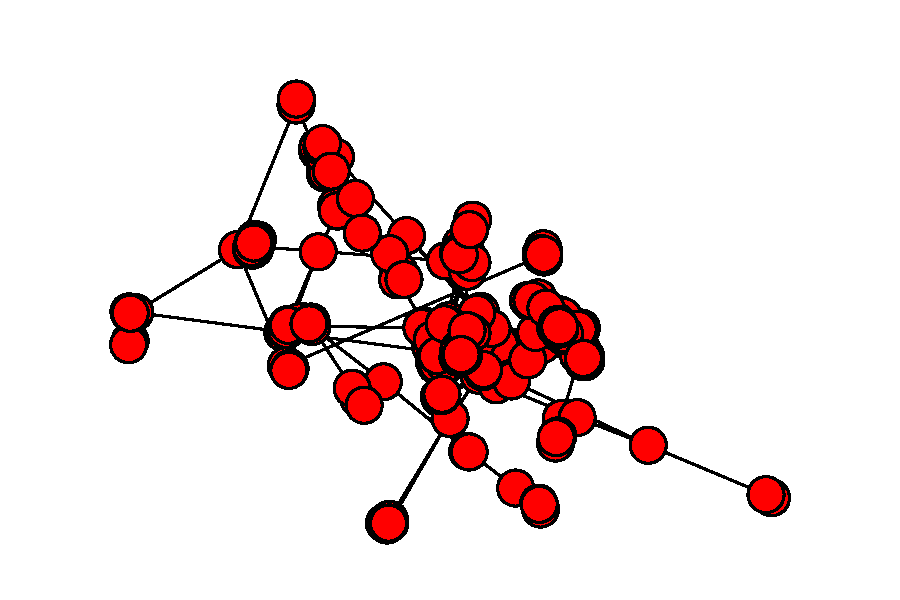
\includegraphics[width=0.5\textwidth]{transactionsNetwork}
  \caption{Maximally Connected Component of Transaction Network: One Hour Prior to Peak Volatility, $8^{th}$ of December 2013}
\end{figure}

\section{Bitcoin \& Blockchain}

Bitcoin is a complex protocol. 
We provide here a brief sketch of the components necessary to understand the analysis presented in this chapter, however due to the many moving parts of the system this is necessarily a superficial overview. 
Interested parties are referred to \cite{narayanan2016bitcoin} for a more complete picture of the system. 

The decentralized currency protocol known as Bitcoin was proposed by Satoshi Nakamoto \cite{nakamoto2008bitcoin}. 
The system utilizes a peer-to-peer (P2P) architecture that enables users to send and receive transactions denominated in units of BTC. 
Users are represented in the network by a public/private key pair. 
Units of BTC can be transmitted to a user by specifying a hash of that user's public key as the receiving party, providing a degree of pseudo-anonymity.  
Users can generate many public keys, i.e. receiving addresses. 
% Secrutiy best practice recommends a new one be used for each transaction. 
The corresponding private keys are used to sign (authorize) transactions. 
Private keys are stored in a ``wallet'' either locally or provided as a hosted service. 

To participate in the Bitcoin network the user runs a client software, such as the Satoshi client, which communicates with a set of peers. 
Transactions are broadcast by the Bitcoin client and received by the peer-to-peer network.
They are confirmed after having been added to the ``blockchain'' - similar to a linked list with the subtle difference that it references the previous block using its hash rather than a pointer. 
This data structure contains blocks of all accepted transactions since the genesis of the system. 

\begin{figure}
\centering
        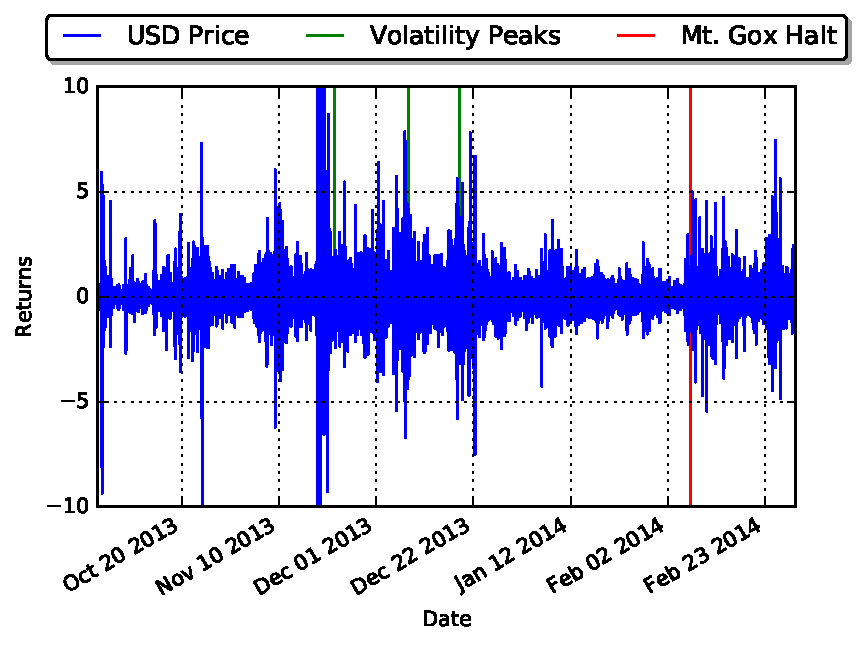
\includegraphics[width=0.6\textwidth]{bitcoinReturns_mtGox}
        \caption{Daily Percentage of Return on Investment}
        \label{fig:RQS}
\end{figure}



Every full node running a Bitcoin client maintains a complete copy of this public blockchain. 
The block generation process confirms new transactions. It necessitates the satisfaction of a computationally expensive ``proof of work'' puzzle. A valid solution to this puzzle entitles the party that deliverers it to the wider network the privilege to issue themselves a reward in the form of newly minted coins. 
The information available through the graph structure of the Bitcoin P2P network is limited due to the dynamic block formation process. 
Each node only has direct knowledge of the peers to which its client is connected. 
The graph of all transactions can be constructed entirely from the publicly available blockchain, wherein the nodes of the graph correspond to Bitcoin addresses and the edges to transactions performed between those addresses. 
In this chapter we empirically study significant global properties of the Bitcoin transaction graph. 

\begin{figure}
\centering
        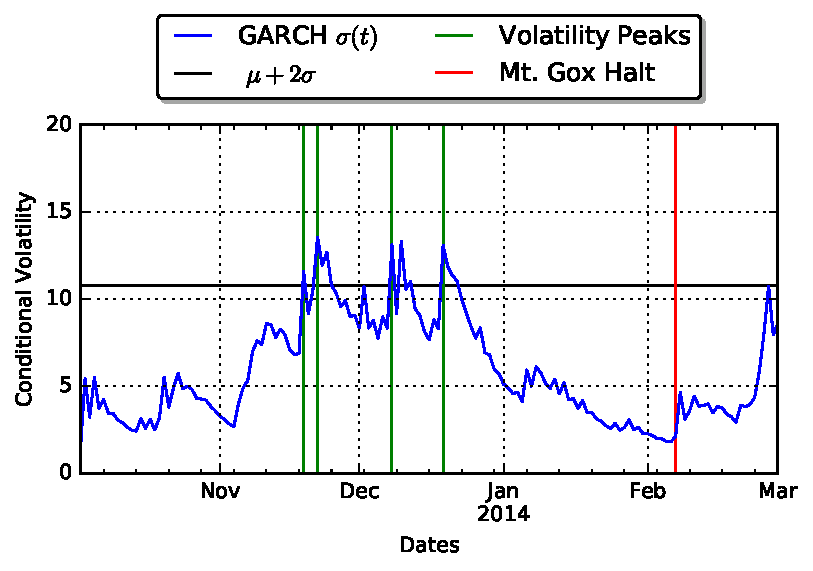
\includegraphics[width=0.8\textwidth]{volatility}
        \caption{Market Volatility}
        \label{fig:PERIODIC}
\end{figure}

\begin{figure}
\centering
        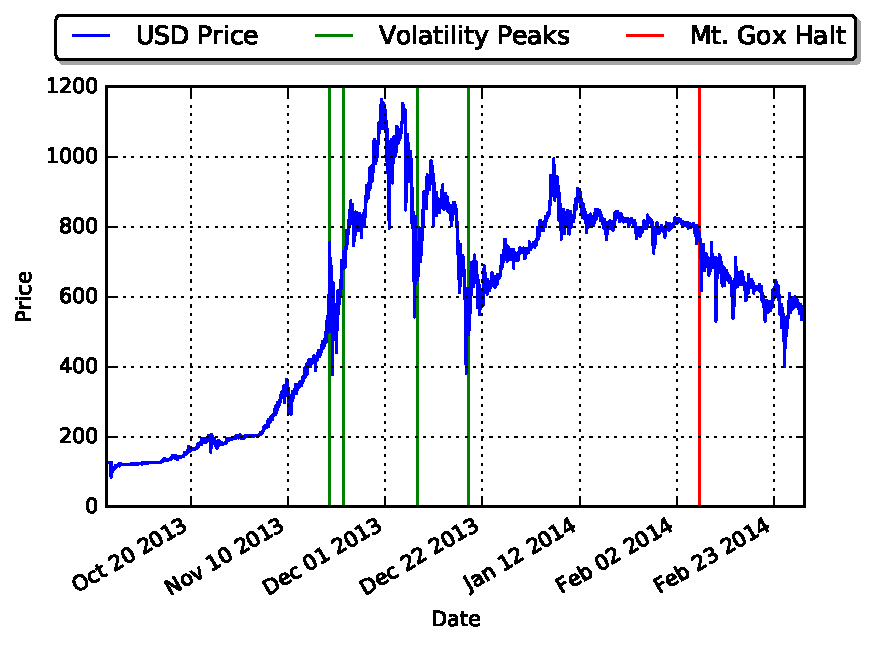
\includegraphics[width=0.8\textwidth]{bitcoinPrice}
        \caption{Bitcoin Price in USD}
        \label{fig:RQL}
\end{figure}
 
With a total market capitalization in excess of \$10,000,000,000 \cite{billy} Bitcoin is the world's largest blockchain-based cryptocurrency. 
The plethora of alternative public blockchain-based cryptocurrencies, many of which are based largely on the open source Bitcoin specification, are amenable to the analyses herein presented.
By a dissection of the full Bitcoin transaction graph throughout four unique phases of exchange activity we discover distinctive characteristics of market pathologies. 

\begin{figure}
\centering
        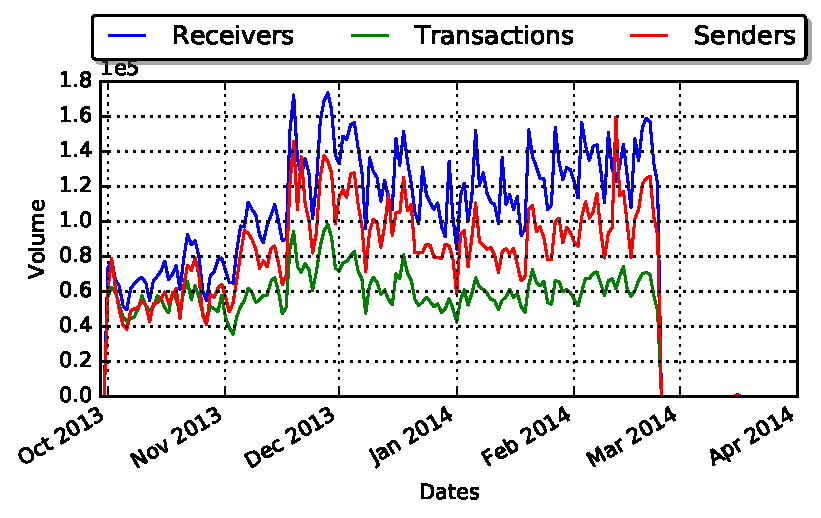
\includegraphics[width=0.6\textwidth]{usersPerDay}
        \caption{Snapshot of Transacting Counter-Parties}
        \label{fig:OU}
\end{figure}

Clustering techniques that associate addresses based on patterns of behaviour degrade the fungibility of individual Bitcoins and in so doing jeopardize the viability of the cryptocurrency as a unit of exchange \cite{moser2014towards}.
As such our work examines addresses on the basis of activity over time, rather than attempting to associate a subset of addresses with a specific identity.
This approach yields insight about network behaviour while preserving the privacy of individual users.

Time series of the USD/BTC exchange rate. We performed a volatility analysis fitting a GARCH model to the returns and established the period of highest market volatitlity through the maximum values of the conditional volatilities as obtained from the model. We show the volume of addresses for both receivers and senders as well as the number of transactions.
% \psfig{file=rosette.ps, height=1in, width=1in,}
Degree distributions for the network of transactions. We can see that the transaction network presents anomalous behavior deviating from Pareto distribution February $5^{th}$ two days before the Mt. Gox transactions halt.

\begin{figure}
  \centering
\begin{lstlisting}[language=json,firstnumber=1]
{
    u'receiver': 
    [  
     {
        u'addr': u'1MZK1SVikQPp2a56cm5q3CPtnwfzNvWyMe', 
        u'value': 17500000000L
     }, 
     {
        u'addr': u'1QJpvMpeuzSoV7nF6u1EVUnDqU7jtBo8Le', 
        u'value': 19980000
     }
    ], 
        u'_id': ObjectId('57fb5ff187a52f69f0ec2802'), 
        u'hash': u'15ccaaaa97790046234e6ef53afcf513cf
        ba2cb1430412b40de544d0fb815a6d', 
        u'senders': 
        [
         {
          u'addr': u'1QJpvMpeuzSoV7nF6u1EVUnDqU7jtBo8Le', 
          u'Value': 19990000
         }, 
         {
          u'addr': u'1CE82aib22UajJ1KtNPTpSH2QKeJZ6o37p',
          u'Value': 17500000000L
         }
        ], 
     u'time': datetime.datetime(2014, 2, 21, 14, 54, 17)
}
\end{lstlisting}
  \caption{Example Data Record}
\end{figure}

\section{Prior Investigations}

The most comprehensive prior treatment of the full (at that time) Bitcoin transaction graph has been conducted by Ron \& Shamir \cite{ron2013quantitative}. 
That analysis considered blocks from January 2009 to May 2012, terminating well before the extreme value fluctuation periods considered in our analysis.
That effort sought to assess statistical properties of the network with a focus on anonymity and the tracking of specific transactions. 
It did not consider structural aspects of the network as a whole as we do in this chapter. 
% Furthermore the time period therein considered terminates well before the extreme value fluctuation periods considered in our analysis. 

Consideration of the Bitcoin transaction network in a time of crisis was undertaken by Donier \& Bouchaud \cite{donier2015markets}, however the data they examine is the order book of Mt. Gox, which was at the time the largest Bitcoin exchange. 
Accordingly, they do not consider the public Bitcoin blockchain data as we do in our treatment. 
Moreover that analysis terminates in January 2014, the month before the collapse of Mt. Gox and the resultant market perturbations that we examine in this chapter. 
The only previous assessment of the Bitcoin bubble of 2013 \cite{garcia2014digital} examines socio-economic signals as opposed to network structure. 
These signals include Twitter data, downloads of the Bitcoin core software client, Google/Wikipedia searches, and prices on various exchanges. 
The work of Ober et. al \cite{ober2013structure} performs an analysis of the transaction graph primarily from the perspective of anonymity and ends before the high volatility periods we examine in this chapter. 
The sole prior work to deal with the crash of Mt. Gox is that of Kristoufek \cite{kristoufek2015main}, which was part of a treatment of the factors that affect the Bitcoin price in terms of speculative activity, considering not blockchain network structure but rather the influence of the Chinese market and technical parameters of the core protocol. 

\begin{figure}
  \centering
    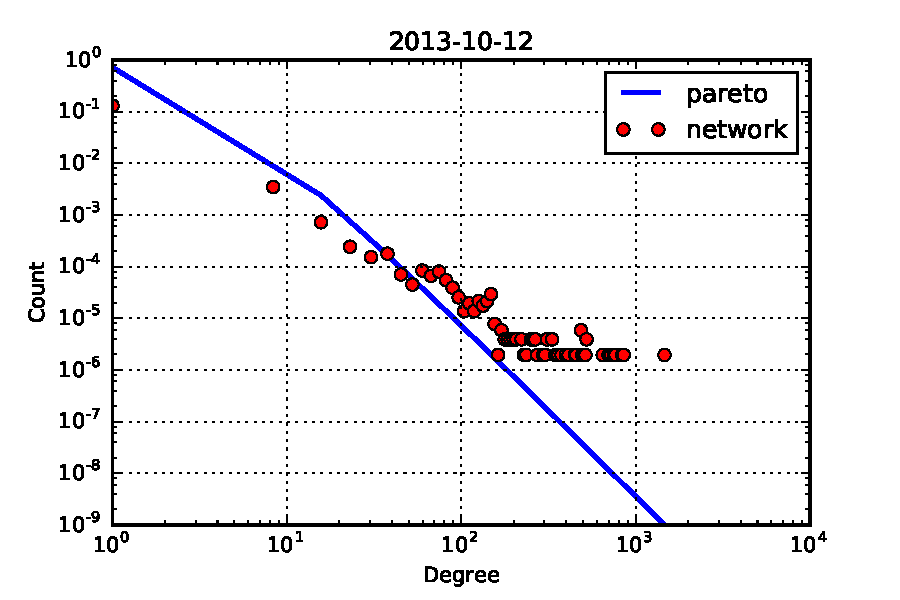
\includegraphics[width=0.8\textwidth]{networkdistribution_2013-10-12_20_30_06.pdf}
  \caption{Normal degree distribution for the network of transactions}
  \label{fig:paretonormal}
\end{figure}

\begin{figure}
  \centering
    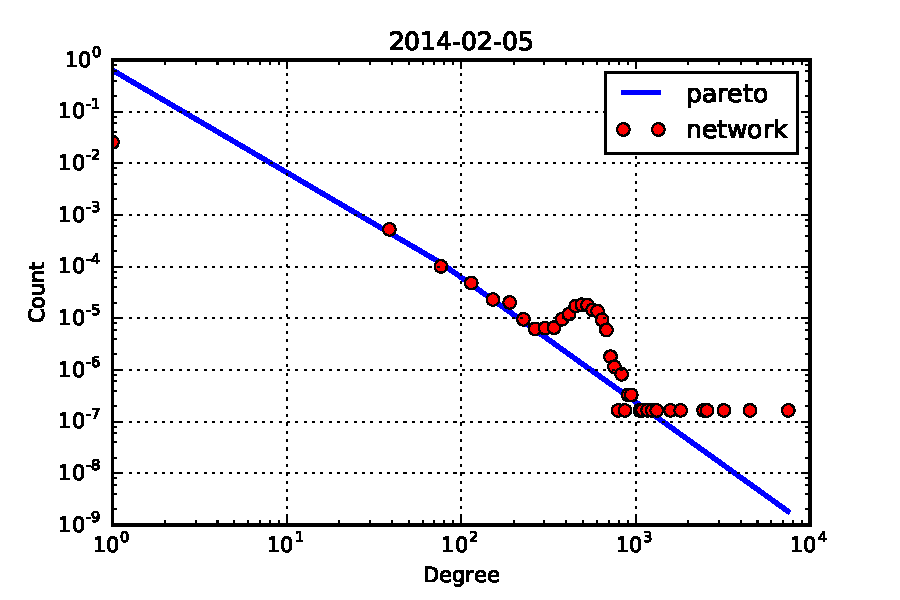
\includegraphics[width=0.8\textwidth]{networkdistribution_2014-02-05_20_30_06.pdf}
  \caption{Mt. Gox degree distribution anomalies}
  \label{fig:anomaly}
\end{figure}

\section{Market Analysis}

% \subsection{Modelling Risk}
In order to characterize the relevant epoch of interest we studied the behavior of the BTC price and performed risk analysis through volatility measures. 
Assessment of risk requires us to define functions of relative uncertainty. 
Volatility catalogs the degree to which the trading price of an asset varies as given by the standard deviation of the return\footnote{Returns here refers to the changes in value of the Bitcoin currency, in our study we use the percent change, or the normalized difference in the prices}. 
Periods of extraordinary market volatility are indicative of high volume fluctuations in nominal value of BTC. We use standard econometric \cite{GARCH} techniques to find the dates of greatest volatility.
Formally, the returns residuals $\epsilon_t$ will be modeled by:

\begin{equation}
\epsilon_t = \sigma_t z_t
\end{equation}

Here $\sigma_t$ represents the standard deviation of the fluctuation at time t and $z_t \sim \mathcal{N}(0,1)$ a noise value at time t, sampled from a normal distribution of mean 0 and variance 1. The index t over $\sigma$ indicates the changes in the fluctuations, $\sigma_t$ is known as the volatility, a measure of the risk in investment, as it quantifies the degree of uncertainty of the future value of the asset. The simplest model for volatility occur in econometrics under the names of ARCH (autoregressive conditional heteroscedasticity) and generalized ARCH (a.k.a GARCH) \cite{GARCH}. Here, heteroscedasticity refers to variations in the fluctuation of the variable of interest, which is in our case $z_t$. Formally, this implies that the covariance $Cov(z_t , z_{t-k})$ depends on time t. The dependence is modeled through past values of the noise $\epsilon_t$ as well as past values of $\sigma_t$.

\begin{equation}
 \sigma^2_t   =  \omega + \sum^{q}_{k=1}\alpha_{k} \epsilon_{t-k}^2 + \sum^{q}_{l=1}\beta_{l} \sigma_{t-l}^2 
\end{equation}

The values of $\alpha_k$, $p$ and $\beta_l$,$q$ determine the correlation of $\sigma_t$ with past fluctuations. For identifying the correct values of the parameters, we fitted the model \footnote{https://pypi.python.org/pypi/arch/3.0} and performed model comparison through Akaike information criteria \cite{Information}.
In generating these models we sought to quantify the degree of market volatility throughout a precisely specified period of time. We show the peaks of high volatility in the Table above.

The highest recorded price of BTC was observed on the $17^{th}$ of November 2013 at \$1,216.73 USD on the exchange Mt. Gox \cite{crash}.
As obtained by volatility analysis we define the \textit{Pre-crash period} and \textit{Post-crash period}, before and after the volatility peak 3.  \textit{Calm period} is given by the first week of January 2014, as it represents stable prices and low fluctuations.
\textit{Pathologies-crash period} on the other hand is given by the first two weeks of February due to volatility and historical knowledge. Mt. Gox halted all Bitcoin withdrawals on the $7^{th}$ of February 2014. Notwithstanding, in each of the other epochs under consideration in our analysis Mt. Gox served as counterparty for the majority of network transactions, at times up to 70\% of all Bitcoin transactions were routed through the platform \cite{wsj}. 


\begin{table}
\centering
\caption{Statistics of Transactions Dataset}
\label{my-label}
\begin{tabular}{|l|c|}
\hline
Sending Addresses:   & 9,951,869  \\ \hline
Receiving Addresses: & 10,447,266 \\ \hline
Total Transactions:  & 8,821,482  \\ \hline
\end{tabular}
\end{table}

In this chapter we take a comprehensive overview of the public blockchain network data.
We examine periods of crisis, such as highly volatile value fluctuations and the implosion of a major financial institution, to discover emergent patterns.  
The epochs considered in this chapter are examined not in terms of classical econometric theory but rather in terms of network structure and empirical analysis. 
The data we use is available as part of the public Bitcoin blockchain as open data.

% \begin{figure}[b]{0.6\textwidth}
%   \centering
%     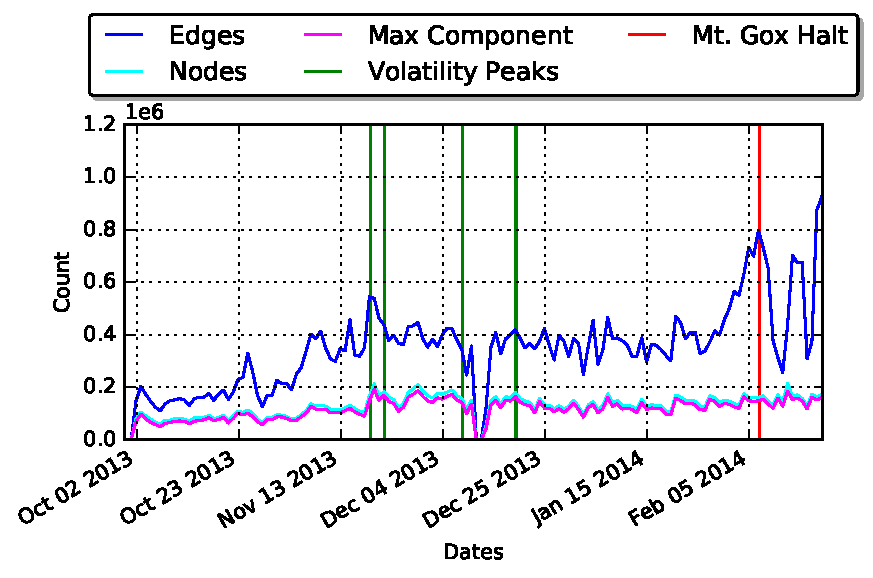
\includegraphics[width=\textwidth]{nodesAndEdges}
%   \caption{Number of Nodes and Edges}
% \end{figure}

% \begin{figure}[b]{0.6\textwidth}
%   \centering
%     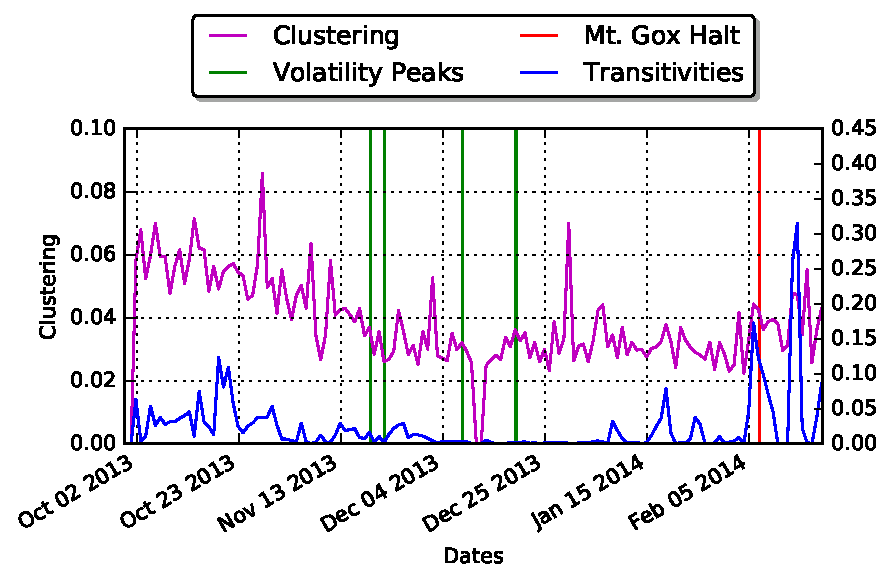
\includegraphics[width=\textwidth]{transitivities}
%   \caption{Transitivities}
%   \label{fig:trans}
% \end{figure}
% Daily values of structural properties in the network of transactions.

\section{Experiment Configuration}

For purposes of our analysis the behavior of the Bitcoin transaction network is grounded by the exchange value of BTC to USD. 
The term \textit{crisis} is used here to describe a period of time wherein the price of BTC suddenly undergoes large fluctuations of nominal value. 
After extended econometric analysis in the above section. We have identified four distinct epochs that portray the Bitcoin transaction network under various conditions of relative stability cataloged in Table 1: Measurement Periods. 

The epochs are labeled according to defining characteristics. \textit{Pre-Crash} is a period of ``irrational exuberance'', that witnessed a general trend towards higher and higher prices. \textit{Post-Crash} entails a precipitous decline in nominal value. \textit{Calm} presents the network under conditions of comparably minor variation in nominal value. \textit{Pathologies-Crash} occurs amidst the implosion of the Mt. Gox exchange, at the time the largest and most central counterparty in the Bitcoin transaction network. We access 28,819 blocks from the Bitcoin blockchain, specifically Block \\ \#260989 of October $1^{st}$ 2013 to Block \#289808 on March $10^{th}$ 2014. From each individual block we extract the transactions. Of each transaction we strip away all data other than the list of inputs and the addresses therein, the list of outputs and the corresponding addresses, and the \texttt{nLockTime}, i.e. the unix time or block number (block height) specifying when the transaction can be accepted into a block. 


\begin{table}
\centering
\label{dates}
\begin{tabular}{|l|c|}
\hline
\multicolumn{2}{|c|}{\textbf{Important Dates}} \\ \hline
\textit{Volatility Peak 1}    & 19 Nov. 2013   \\ \hline
\textit{Volatility Peak 2}    & 22 Nov. 2013   \\ \hline
\textit{Volatility Peak 3}    & 08 Dec. 2013   \\ \hline
\textit{Volatility Peak 4}    & 19 Dec. 2013   \\ \hline
\textit{Mt. Gox Halt}         & 7 Feb. 2014    \\ \hline
\end{tabular}
\end{table} 


The total number of transactions in this set is 8,821,482. We make a distinction between sending addresses, of which there are 9,951,869 and receiving addresses of which there are 10,447,266. This is logically consistent with our expectations due to the concept of a ``change address'' whereby remaining UTXO outputs are assigned to the private key responsible for generating the transaction, thus ensuring that there are typically a higher percentage of receivers in the network than senders. 

% OOOOOOOOOOOOOOOOOOOOOOOOOOOOOOOOOOOOOOOOOOOOOOO
% ooooooooooooooooooooooooooooooooooooooooooooooo
% -----------------------------------------------
% Our network structure analysis was conducted using ASK CESAR WHAT WE USED!

% -basic pareto information

% -explaining the network analysis stuf in high level terms






\begin{table}
\centering
\caption{Measurement Periods}
\label{table:my-label}
\begin{tabular}{|l|c|c|}
\hline
\textbf{Epoch Name:}            & \multicolumn{1}{l|}{\textbf{Begin:}} & \multicolumn{1}{l|}{\textbf{Terminate:}} \\ \hline
\textit{Pre-Crash}         & $1^{st}$ Nov. 2013                          & $6^{th}$ Dec. 2013                              \\ \hline
\textit{Post-Crash}        & $8^{th}$ Dec. 2013                          & $28^{th}$ Dec. 2013                             \\ \hline
\textit{Calm}              & $15^{th}$ Jan. 2014                         & $31^{st}$ Jan. 2014                             \\ \hline
\textit{Pathologies-Crash} & $1^{st}$ Feb. 2014                          & $15^{th}$ Feb. 2014                             \\ \hline
\end{tabular}
\end{table}






% Times of economic panics and crises are exaserbated by uncertainty and lack of confidence. 
% The transparency inherent in blockchain-based cryptocurrencies presents a model whereby access to a complete picture of the transaction network exposed via APIs. 
% It has been said that data is a new natural resource.
% These transactions are one important part of thwarting economic crises the other indispensible component is sophisticated analytical tools. 
% To create an index of market instability we access the information associated with the most severe economic crisis in the history of the Bitcoin currency. 

% For this purpose we accessed 28,819 blocks from the Bitcoin blockchain, specifically Block \#260989 of October $1^{st}$ 2013 to Block \#289808 on March $10^{th}$ 2014. 
% These blocks were further partitioned into four distinct Measurement Periods or epochs that encapsulate particular network structures describing unique configurations of market conditions. 

% The total number of transactions in this set is 8,821,482.
% We make a distinction between sending addresses, of which there are 9,951,869 and receiving addresses of which there are 10,447,266.
% This is logically consistent with our expectations due to the concept of a change address whereby remaining UTXO outputs are reassigned to the private key responsible for generating the transaction. 
% Thus ensuring that there are typically a higher percentage of receiving parties in the network than senders. 

% The term crisis is used here to describe a situation wherein the price of BTC suddenly loses a large percentage of nominal value. 

% data record
% The Bitcoin blockchain encodes transactions together with significant meta-data. 
% For our purposes this was pruned to extract only information applicable to our analysis, as demonstrated by Figure 3.


\section{Economic Distortions}


The Bitcoin network supports a wide variety of market activity.
Small time market participants, less than 50 transactions in the epochs described by our dataset, were excluded from the analysis of the market pathology. 
Accordingly those results are applicable to market actors that receive and transmit a relatively high number of transactions on a consistent basis.
Representative examples of these players include the following: 
\begin{itemize}
  \item Online gambling platforms such as \texttt{SatoshiDice}\footnote{\texttt{http://www.satoshidice.com}} which provide entertainment.
  \item Media outlets including \texttt{CoinTelegraph}\footnote{\texttt{http://www.cointelegraph.com}} that compensate journalists using BTC.  
  \item Darknet markets accessible over the Tor network such as \texttt{AlphaBay Market}\footnote{\texttt{http://pwoah7foa6au2pul.onion}}, providing an auction and corresponding reputation system. 
  \item Purveyors of financial instruments, e.g. binary options purchasable through \texttt{BTC Oracle}\footnote{\texttt{http://www.btcoracle.com}}.
  \item Exchanges including \texttt{Kraken}\footnote{\texttt{http://www.kraken.com}} that serve as a bridge between the fiat economies (USD, EUR, etc.), and as a platform for exchanging between alternative cryptocurrencies such as Litecoin. 
\end{itemize}

In order to gain insight into the mechanism which induced the network distortion we performed an exhaustive analysis of the dynamical patterns for each individual address, and for each characteristic epoch as defined in relevant Table.  
We define a dynamical vector as the hourly departure, i.e. transmission of BTC, volumes for each address.

In order to avoid the curse of dimensionality and uncover relevant dynamical characteristics, we performed dimensionality reduction of the vector matrices through PCA decomposition. 
We subsequently cluster the points with the k-means algorithm. 
The results are presented in the Figure for each of the epochs.

% \begin{figure}
%   \centering
%     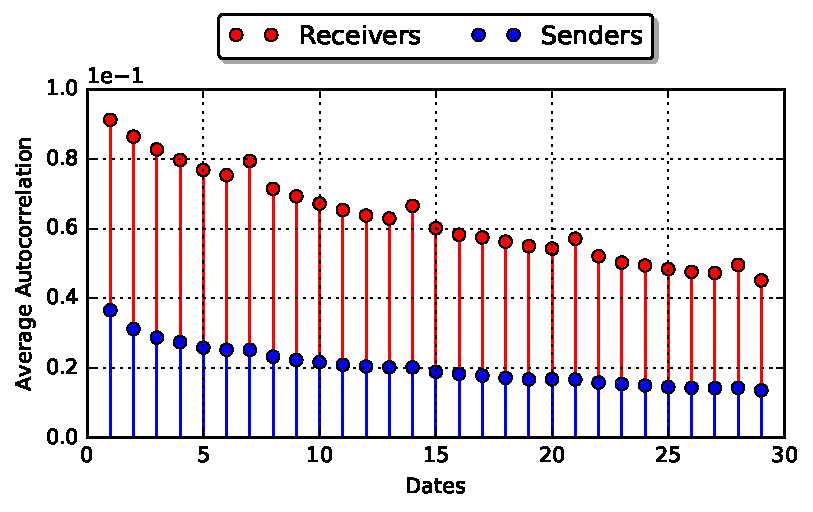
\includegraphics[width=0.3\textwidth]{usersAutoCorrelations}
%   \caption{Auto correlation function of the addresses}
%   \label{fig:auto}
% \end{figure}

% \begin{figure}
%   \centering
%     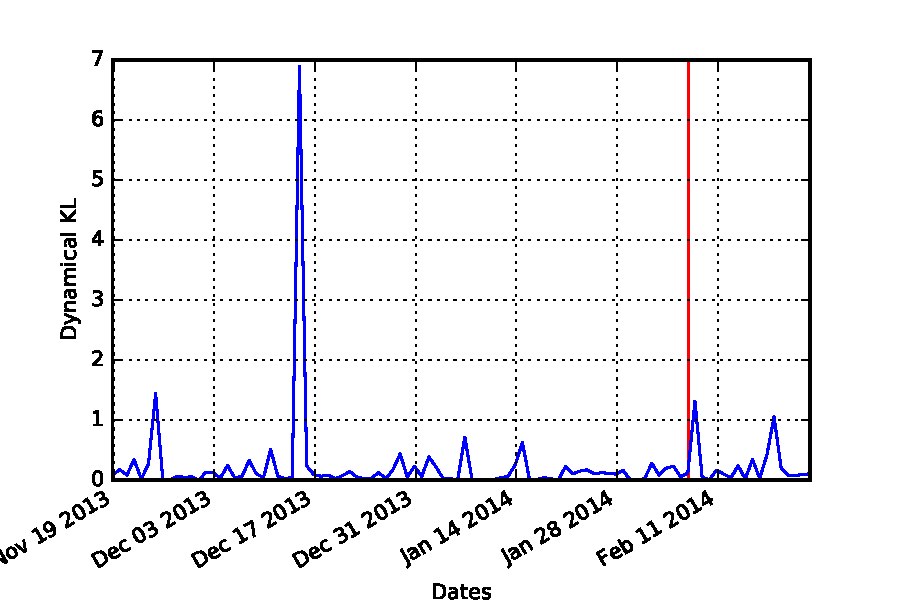
\includegraphics[width=0.3\textwidth]{KL.pdf}
%   \caption{DiscoPath metric for the time period studied. The biggest peaks represent the volatility regions and the Mt. Gox anomalies as pointed out by the red line}
% \end{figure}


The \textit{Pre-crash period} is described by three primary clusters of activity.
The largest of which is represented by a relatively sparse dispersion of departure points.
In contrast the two complimentary clusters of the \textit{Pre-crash period} both feature high volumes of departures that occur with short inter-departure times.
The epoch denoted \textit{Post-crash period} features only two clusters, indicating that the more dense cluster (Red circle), clearly discernible in the other epochs, has been fully absorbed. 
The largest cluster has markedly changed from a sparse dispersion of departures to one punctuated by a 10-fold increase in frequency.
This indicates a waiting period of less duration between transactions.
The decrease in latency between transmission executions is indicative of the variation in the return residual. 
\textit{Pathologies-crash period} corresponds to the long-tail anomaly of Figure 4b. 
We observe in the green cluster an atypically high concentration of send activity over the course of only two days, recall that this is the depiction of a cluster representative i.e. the associated cluster points share the same activity pattern, though not necessarily at the same moment in time. 
This indicates that the cluster point is transmitting BTC to many different addresses in a short time frame. 
The result is high degree connectivity among nodes in the network, induced dynamically. 
This process generates a bifurcation in the cluster structure, in contrast to the ``\textit{stretched}'' structure of the other epochs. 
The \textit{Calm period} is similar in composition to that of the \textit{Pre-crash period}, as it has three distinct clusters and is characterized by relative uniformity in the transmission profile of the cluster representatives.

We seek to define reliable metrics which capture the underlying nature of the meta-data we are analyzing. 
As revealed by the empirical analysis in our description of economic distortions we seek to incorporate both the dynamical as well as the structural component of the observed phenomena. 
We do so by focusing our attention on the unexpected changes in the degree distribution of the daily network of transactions $P_i(k)$. 
The key principle underlying our approach is that, as observed, periods of market distortions are characterized by changes in the \textit{baseline} Pareto distribution.
In times of market fluctuations or anomalies,  the observed distributions $Q_i(k)$ posses a markedly different distribution shape. 

A common approach used to study differences between two distribution $P$ and $Q$ is through the Kullback Leibler divergence  KL(P||Q) \footnote{Referred to also as the relative entropy or the information divergence.}  \cite{Information}.
Intuitively we can understand this distribution as encoding the likelihood that  $P$  produced data from itself, as opposed to the likelihood that it is produced by $Q$ \cite{sloppiness}. 
To incorporate the dynamical aspect, we study the delayed divergence. 
Finally we have:

\begin{equation}
KL(P_{i-1}(k) || Q_i(k)) = \sum_{j}P_{i-1}(k_j)\log{\frac{P_{i-1}(k_j)}{Q_i(k_j)}}
\end{equation}

We call this  metric the ``\textit{DiscoPath}'' (Figure 4b). This formulation possesses several advantages. 
One of which is the encapsulation of the dynamical locality in the sense that we are measuring against the one day delay pattern \textit{baseline} Pareto distribution. 
We would expect a different definition of what the \textit{baseline} is as the market evolves. 
The parameter configuration of a single day delay allows us to uncover both the start and the end of the pathology. 
As the network drifts back to a more typical structural distribution there will be a ``jump''  indicative of the anomaly.

\section{Reflection}

The primary contribution of this chapter is the definition of a metric to recognize perturbations in the transaction networks of public blockchain-based cryptocurrencies such as Bitcoin. 
We performed standard econometric analysis in order to classify different epochs of the blockchain history. 
Further we study basic behavior of the addresses through the autocorrelation function, we then introduced undirected networks upon which we performed network theory analysis.
We found distinctive behavior in the clustering and transitivity of the network, with low values for highly volatile periods and high values after the Mt. Gox crisis. 
After observing the deviations in Pareto behavior, we defined a information theory metric in order to quantify and follow such deviations.

In the time since the epochs examined herein the Bitcoin network has stabilized considerably. 
The network does however remain fraught with smaller scale ``micro-crashes'' and future extensions to our system entail an enhancement of appreciable time scale granularity to facilitate the application of our network to predict more common market anomalies. 
These results are part of an ongoing program of research.
Planned extensions to the work presented include enrichment with geographic information, as well as the definition of a weighted network through the application of transaction amounts to edges between nodes.

Blockchain-based cryptocurrencies on the model of Bitcoin maintain a publicly available record of all the transactions conducted on the network. 
This represents a fundamentally new way of organizing the so-called ``back-end'' processes of a web-scale service. 
The information thus recorded is available to anyone with the interest to examine it, without the strictures of an API limit or a restrictive licensing agreement.
Cryptocurrencies are the first application to fully embrace this model. 
If other web-scale services, such as large search engines or micro-blogging platforms, were to follow suit and organize around a similar model of open data it holds the potential to herald a renaissance in the field of network analytics.  

The Bitcoin model first emerged in the midst of the greatest financial crisis weathered by the traditional economy in living memory. 
The science fiction author William Gibson remarked that ``\textit{when you want to know how things really work, study them when they're coming apart}''.
Accordingly in this analysis we study the Bitcoin network amidst its own time of coming apart, the great bubble of 2013 and the spectacular dissolution of Mt. Gox, the largest and most central financial institution. 
From this time of turbulence we have extracted DiscoPath, a mechanism for the discovering of pathologies, i.e. significant deviations from the typical Pareto distribution of BTC to addresses.
By these means we seek to recognize the manifestation of similar crises in the days, weeks, months, and years to come.

% In this analysis the Bitcoin blockchain afforded us the opportunity to carry-out an exhaustive post-mortem on one of the most severe financial crises to befall this nascent cryptocurency.
% Economists have heretofore endeavored to employ ever more creative mechanisms to infer the behavior of economic actors within a monetary system. 
% The Bitcoin blockchain puts the raw information of value exchange at the fingertips of any and all interested parties. 
% This work represents an initial endeavor into the realm of rigorous network scientific inference of economic principles from an operational cryptocurrency based on a Bitcoin-esque (viz. blockchain) data-structure.



